% ============================================================
% Lecture deck — Module 8 / Notebook 29
% BPM, Governance, POC -> MVP -> Production. HSBI house style. TikZ.
% The notebook is the single source of truth.
% ============================================================
\documentclass[aspectratio=169,11pt]{beamer}

\usepackage[utf8]{inputenc}
\usepackage[T1]{fontenc}
\usepackage{lmodern}
\usepackage[english]{babel}
\usepackage{graphicx}
\usepackage{booktabs}
\usepackage{amsmath,amssymb}
\usepackage{xcolor}
\usepackage{tikz}
\usetikzlibrary{positioning,arrows.meta,shapes.geometric,calc,fit,backgrounds}

\usetheme{Madrid}
\usecolortheme{default}
\setbeamertemplate{navigation symbols}{}
\setbeamertemplate{footline}[frame number]
\setbeamertemplate{blocks}[rounded][shadow=false]
\setbeamertemplate{headline}{%
  \leavevmode%
  \hbox{%
    \begin{beamercolorbox}[wd=\paperwidth,ht=2.5ex,dp=1.125ex]{section in head/foot}%
      \insertsectionnavigationhorizontal{\paperwidth}{}{\hskip0pt plus1filll}%
    \end{beamercolorbox}%
  }%
}
\AtBeginSection[]{%
  \begin{frame}{Outline}
    \tableofcontents[currentsection,sectionstyle=show/shaded,subsectionstyle=show/show/hide]
  \end{frame}
}

\definecolor{hsbiblue}{RGB}{45,57,120}
\definecolor{hsbimid}{RGB}{76,114,176}
\definecolor{hsbilight}{RGB}{225,231,247}
\definecolor{cgreen}{RGB}{85,164,103}
\definecolor{corange}{RGB}{221,132,82}
\definecolor{cred}{RGB}{196,78,82}
\definecolor{cpurple}{RGB}{129,114,178}
\tikzset{
  box/.style={rounded corners=3pt, draw=hsbiblue, line width=1pt, fill=hsbilight, align=center, inner sep=5pt, font=\footnotesize},
  phase/.style={rounded corners=3pt, draw=hsbiblue, line width=1.1pt, fill=hsbilight, align=center, text width=2.1cm, minimum height=0.95cm, font=\scriptsize},
  stage/.style={rounded corners=3pt, draw=hsbiblue, line width=1.2pt, align=center, text width=3.2cm, minimum height=1.6cm, font=\scriptsize},
  arr/.style={-{Stealth[length=2.6mm]}, line width=1pt, draw=hsbiblue},
}

\title{BPM, Governance, and POC $\to$ MVP $\to$ Production}
\subtitle{Module 8 --- Business AI in Practice $\cdot$ Notebook 29}
\author{Prof.\ Dr.\ Christoph Weisser}
\institute{HSBI}
\date{Summer Semester 2026}

\begin{document}

\begin{frame}\titlepage\end{frame}

\begin{frame}{Contents}
  \tableofcontents[hideallsubsections]
\end{frame}

% ============================================================
\section{BPM}
% ============================================================
\begin{frame}{Embedding AI in the BPM lifecycle}
  \begin{center}
  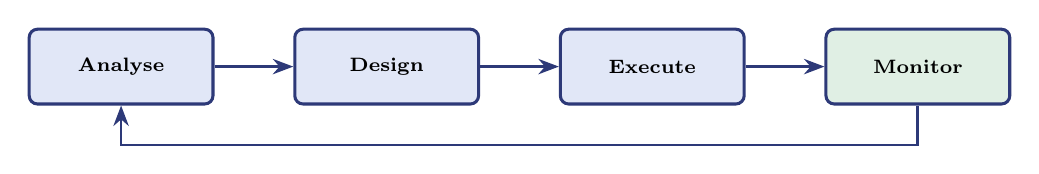
\begin{tikzpicture}
    \node[phase] (a) {\textbf{Analyse}};
    \node[phase, right=1.0cm of a] (d) {\textbf{Design}};
    \node[phase, right=1.0cm of d] (e) {\textbf{Execute}};
    \node[phase, right=1.0cm of e, fill=cgreen!18] (m) {\textbf{Monitor}};
    \draw[arr] (a)--(d); \draw[arr] (d)--(e); \draw[arr] (e)--(m);
    \draw[arr] (m.south) -- ++(0,-0.5) -| (a.south);
  \end{tikzpicture}
  \end{center}
  \begin{exampleblock}{Tip --- name the phase before you scope the work}
    When a stakeholder pitches an AI project, ask which BPM phase it lands in. If they can't say, the project is still a \emph{wish}, not a feature.
  \end{exampleblock}
\end{frame}

% ============================================================
\section{Governance}
% ============================================================
\begin{frame}{Governance --- a RACI for an AI initiative}
  \begin{block}{RACI, extended so the \emph{AI system} is a named actor}
    Responsible $\cdot$ Accountable $\cdot$ Consulted $\cdot$ Informed.
  \end{block}
  \begin{itemize}
    \item The AI is \textbf{R} for an \emph{individual} decision --- but a human is always \textbf{A}. The AI cannot be blamed.
    \item \textbf{Compliance is A} for the provider choice --- anything touching customer data has a veto.
    \item \textbf{Rollback is owned by the platform team}: ML decides \emph{whether} to revert; platform can actually \emph{do} it.
  \end{itemize}
\end{frame}

% ============================================================
\section{POC to Prod}
% ============================================================
\begin{frame}{POC $\to$ MVP $\to$ Production --- three projects, not three phases}
  \begin{center}
  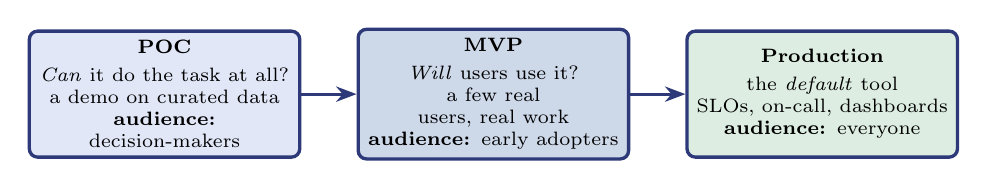
\begin{tikzpicture}
    \node[stage, fill=hsbilight]  (p) {\textbf{POC}\\[2pt] \emph{Can} it do the task at all?\\ a demo on curated data\\ \textbf{audience:} decision-makers};
    \node[stage, fill=hsbimid!28, right=0.7cm of p] (m) {\textbf{MVP}\\[2pt] \emph{Will} users use it?\\ a few real users, real work\\ \textbf{audience:} early adopters};
    \node[stage, fill=cgreen!20, right=0.7cm of m] (pr) {\textbf{Production}\\[2pt] the \emph{default} tool\\ SLOs, on-call, dashboards\\ \textbf{audience:} everyone};
    \draw[arr] (p)--(m); \draw[arr] (m)--(pr);
  \end{tikzpicture}
  \end{center}
  \begin{alertblock}{The most common confusion}
    Production is \emph{not} ``MVP, but more robust.'' It is MVP \emph{plus all the boring operational work} --- monitoring, rollback, cost control, support.
  \end{alertblock}
\end{frame}

% ============================================================
\section{Cases}
% ============================================================
\begin{frame}{Three case studies --- what real initiatives look like}
  \begin{itemize}
    \item \textbf{Triage \textcolor{cgreen}{(shipped)}.} The classifier wasn't the hard part --- ticketing integration, queue routing, and the override UI were. The provider shim and monitoring both paid off.
    \item \textbf{Invoice processing \textcolor{cgreen}{(shipped)}.} The AI was \emph{30\,\%} of the project; ingestion, ERP integration, and the review UI were the other 70\,\%. Trust grew from \emph{observation}; a rule layer caught hallucinated invoice numbers.
    \item \textbf{Sales analytics \textcolor{cred}{(did not ship)}.} A solution looking for a problem --- never a specific user story. \emph{Discovery is allowed to conclude ``don't build it.''}
  \end{itemize}
\end{frame}

% ============================================================
\section{Checklist}
% ============================================================
\begin{frame}{A one-page readiness checklist}
  \footnotesize
  \begin{block}{Ten questions a technical lead uses to say ``no'' constructively}
    \begin{enumerate}
      \item \textbf{User} --- who \emph{specifically} uses it?
      \item \textbf{Task} --- which task does it absorb? (name it with a verb)
      \item \textbf{BPM phase} --- analyse / design / execute / monitor?
      \item \textbf{Pattern $\times$ stake} --- where on the 2$\times$2 from Notebook 26?
      \item \textbf{Baseline} --- how is the task done today, and how long does it take?
      \item \textbf{Success metric} --- what number is measurably different in 8 weeks?
      \item \textbf{Failure mode} --- what does a wrong answer look like, and who notices?
      \item \textbf{Rollback} --- can you switch it off in 5 minutes?
      \item \textbf{Cost model} --- per-call cost, and the implied monthly bill at full scale?
      \item \textbf{RACI} --- who is A for runtime, compliance, and rollback?
    \end{enumerate}
  \end{block}
  {\footnotesize Full detail, the RACI table, and the three cases end-to-end are in \textbf{Notebook 29}.}
\end{frame}

\end{document}
